
\subsection{Densitat de malla}

La densitat de malla és el nombre de volums de control i de nodes en què discretitza espacialment el domini. Es diu que la malla és grollera si la discretització té pocs volums de control i es diu és fina si en té molts. Intuïtivament, una malla més fina donarà resultats més pròxims a la realitat.

Per l'anàlisi de la densitat de malla es pren una discretització uniforme, donada per la condició \eqref{eq:malla_uniforme}, i es fixa el valor de $N_1$, amb $N_1 \in \{ 5, \, 15, \, 25, \, 35, \, 45, \, 55\}$. L'esquema d'integració numèrica és Crank--Nicolson, amb $\Delta t = 1.00 \ \second$. Es calculen els mapes de temperatura en $t = 5000 \ \second$ i $t = 10000 \second$. La condició de convergència és $\delta = 10^{-11}$. 

En les representacions dels mapes de temperatura no s'interpola entre nodes dels nodes, sinó que cada volum de control té assignada la temperatura del seu node. El motiu d'aquesta decisió es mostra a la figura \ref{fig:malla_comparacio}.
\begin{figure}[ht]
	\centering
	\begin{subfigure}{.5\textwidth}
		\centering
		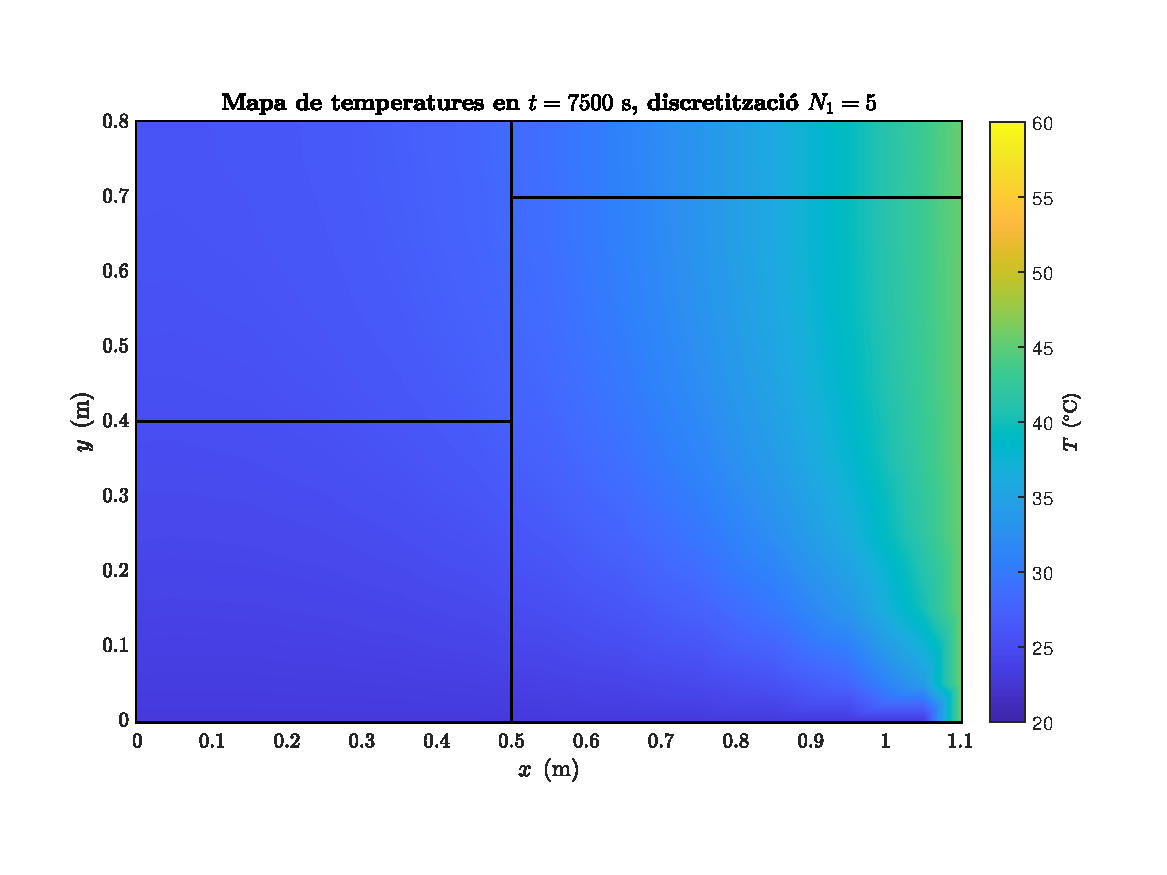
\includegraphics[width=.95\linewidth]{imagenes/04_analisi_influencia_dades_numeriques/malla/malla_31.pdf}
		\vspace{-15pt}
		\caption{Temps $t_\text{max} = 7500 \ \second$, discretització $N_1 = 5$.}
		\label{fig:malla_31}
	\end{subfigure}%
	\begin{subfigure}{.5\textwidth}
		\centering
		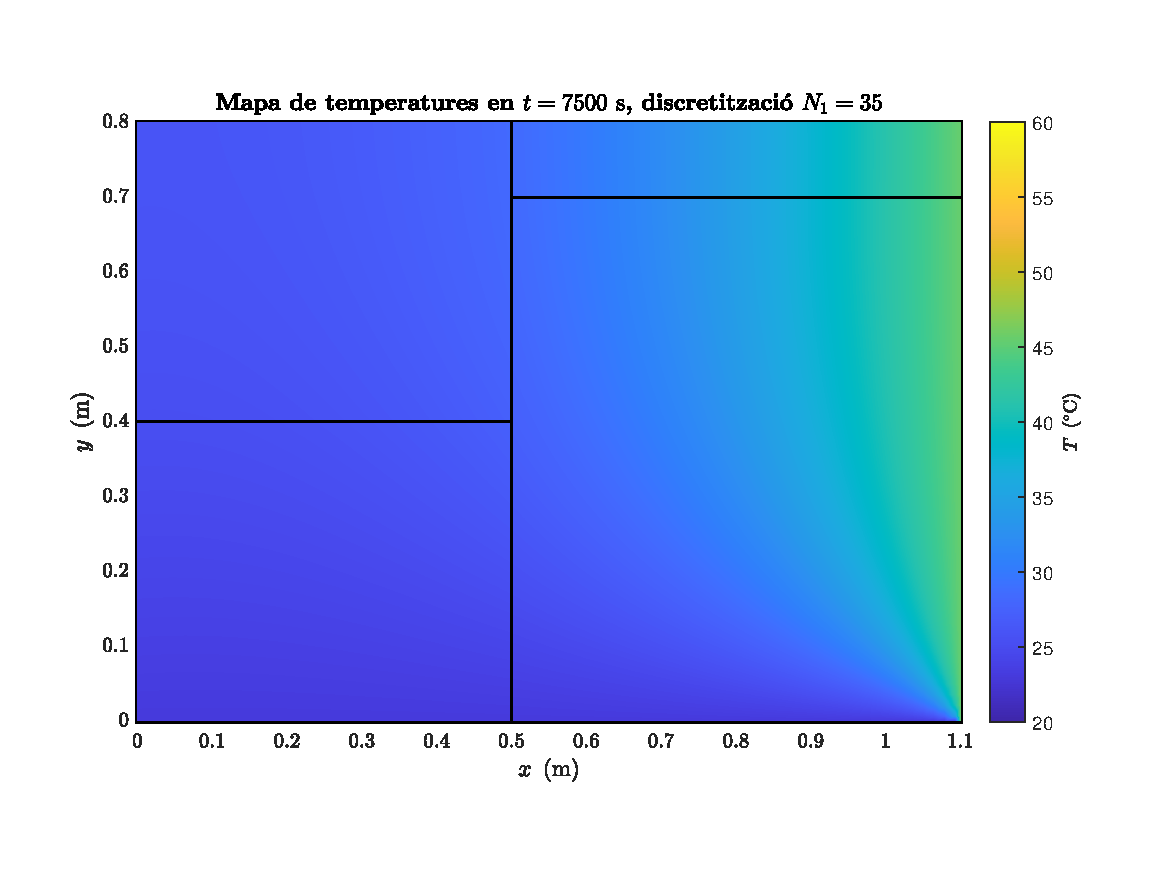
\includegraphics[width=.95\linewidth]{imagenes/04_analisi_influencia_dades_numeriques/malla/malla_34.pdf}
		\vspace{-15pt}
		\caption{Temps $t_\text{max} = 7500 \ \second$, discretització $N_1 = 35$.}
		\label{fig:malla_34}
	\end{subfigure}
	\caption{Mapes de temperatures en $t_\text{max} = 7500 \ \second$ i discretitzacions de $N_1 = 5$ i $35$ nodes, amb interpolació.}
	\label{fig:malla_comparacio}
\end{figure} 

\noindent
La discretització amb $N_1 = 35$ és molt més fina que la corresponent a $N_1 = 5$. Conseqüentment ha de donar millors resultats. Com s'observa, si s'interpola la temperatura entre nodes, aquesta diferència no s'aprecia.

Per a les diferents discretitzacions considerades, a les figures \ref{fig:malla_5000} i \ref{fig:malla_10000}, es mostren els mapes de temperatures en $t = 5000 \ \second$ i $t = 10000 \ \second$, respectivament. En vista dels resultats obtinguts, es conclou que una discretització uniforme no és adequada. Donat que el gradient de temperatures en els materials $M_1$ i $M_3$ és petit, no és necessària una discretització tan fina. En canvi, a la paret dreta el gradient de temperatures es major, requerint de major finor en la malla.

